\section{Results}
\label{sec:results}

\subsection{The architecture does not generalize on its own}
\label{sec:res-architecture}

Before any task training, we score the held-out suite using only the
output format and a pretrained backbone.

\begin{center}
\begin{tabular}{llr}
\toprule
backbone & configuration & held-out mean \\
\midrule
encoder, 150M   & pretrained masked-LM head at the marker & 0.7$\times$ chance \\
encoder, 395M   & same readout, larger model              & 2.2$\times$ chance \\
\midrule
decoder, 1.7B   & state and options concatenated plainly  & 0.8$\times$ chance \\
decoder, 1.7B   & \quad + each option framed as yes/no    & 2.9$\times$ chance \\
decoder, 1.7B   & \quad + a preamble stating the task     & \textbf{11.5$\times$ chance} \\
decoder, 1.7B   & \quad \emph{control:} shortened framing & 5.7$\times$ chance \\
\bottomrule
\end{tabular}
\end{center}

The two halves of the table are different backbones and are not directly
comparable; each is internally consistent. Within the encoder rows, a
strong bidirectional model with a clever output format scores \emph{below
chance} and its larger sibling barely clears it. Within the decoder rows,
the format is worth an order of magnitude.

The last row is the control that matters: shortening the framing to
\texttt{\{opt\}\textbackslash ncorrect? answer} roughly halves the mean,
so the gain is the format doing work rather than an incidental wording
choice.

The same sensitivity appears in option rendering. On the held-out binary
task, scoring the two \noul{} descriptions rather than bare polarity costs
AUROC $0.63$ against $0.712$, because the descriptions restate one
judgement from opposite sides and a model scoring both measures their
overlap.

\subsection{Held-out transfer}
\label{sec:res-heldout}

Table~\ref{tab:heldout} gives the final encoder trained on the audited
279-task mixture. Harness sanity $1.000$; held-in control $1.1$--$2.3\times$.

\begin{table}[t]
\centering
\begin{tabular}{lrrrcr}
\toprule
task & $K$ & chance & accuracy & 95\% CI & $\times$ chance \\
\midrule
\texttt{clinc\_oos}      & 151 & 0.007 & 0.628 & [0.587, 0.672] & \textbf{94.9} \\
\texttt{massive\_intent} &  60 & 0.017 & 0.473 & [0.430, 0.512] & \textbf{28.4} \\
\texttt{banking77}       &  77 & 0.013 & 0.290 & [0.255, 0.323] & \textbf{22.3} \\
\texttt{ag\_news}        &   4 & 0.250 & 0.735 & [0.698, 0.772] & 2.9 \\
\texttt{sst5}            &   5 & 0.200 & 0.412 & [0.373, 0.452] & 2.1 \\
\texttt{civil\_comments} &   2 & 0.500 & 0.683 & [0.648, 0.718] & 1.4 \\
\texttt{helpsteer}       &   5 & 0.200 & 0.262 & [0.225, 0.297] & 1.3 \\
\midrule
\multicolumn{5}{l}{mean multiple of chance} & \textbf{21.9} \\
\bottomrule
\end{tabular}
\caption{Held-out transfer, 600 rows per task, never trained on. The suite
began this work at 0.9$\times$ chance. Every interval excludes its chance
floor.}
\label{tab:heldout}
\end{table}

\paragraph{One task is weaker than the table implies.} Against the
majority-class baseline rather than $1/K$, \texttt{civil\_comments} wins
outright ($0.683$ vs $0.500$, $p<10^{-15}$) but \texttt{helpsteer} sits on
the line: $0.262$ against a $0.233$ baseline, $p = 0.050$. Six of seven
are unambiguous; the seventh beats chance while only matching the trivial
baseline. The decoder of Section~\ref{sec:res-declora} removes this
caveat.

\subsection{A LoRA decoder transfers substantially better}
\label{sec:res-declora}

The same mixture, the same augmentation, rank-16 adapters on
Qwen3-1.7B instead of the encoder. This was the experiment our
pre-registered ablation plan named as deciding the architecture, and it
decides it clearly. Harness sanity $1.000$; held-in control
$1.5$--$2.5\times$, against the encoder's $1.1$--$2.3\times$.

\begin{table}[t]
\centering
\begin{tabular}{lrrcrr}
\toprule
task & $K$ & accuracy & 95\% CI & $\times$ chance & encoder \\
\midrule
\texttt{clinc\_oos}      & 151 & \textbf{0.783} & [0.752, 0.817] & \textbf{118.3} & 0.628 \\
\texttt{massive\_intent} &  60 & \textbf{0.773} & [0.738, 0.805] & \textbf{46.4}  & 0.473 \\
\texttt{banking77}       &  77 & \textbf{0.728} & [0.693, 0.765] & \textbf{56.1}  & 0.290 \\
\texttt{ag\_news}        &   4 & 0.803 & [0.772, 0.838] & 3.2  & 0.735 \\
\texttt{sst5}            &   5 & 0.438 & [0.400, 0.475] & 2.2  & 0.412 \\
\texttt{civil\_comments} &   2 & 0.688 & [0.655, 0.727] & 1.4  & 0.683 \\
\texttt{helpsteer}       &   5 & 0.282 & [0.247, 0.320] & 1.4  & 0.262 \\
\midrule
\multicolumn{4}{l}{mean multiple of chance} & \textbf{32.7} & 21.9 \\
\bottomrule
\end{tabular}
\caption{Held-out transfer, LoRA decoder against the encoder on identical
data and identical items. Every task improves.}
\label{tab:declora}
\end{table}

Two results matter here beyond the mean. First, \textbf{every task now
beats its majority-class baseline}, not merely $1/K$: \texttt{helpsteer}
reaches $0.282$ against $0.233$ at $p = 0.0025$, removing the single
caveat that qualified the encoder result. Second, \textbf{Banking77
zero-shot rises from $0.290$ to $0.728$} against the commercial
reference's $0.820$. A fifty-three point deficit becomes nine.

\paragraph{The architecture decision.} Our ablation registry fixed three
possible outcomes before this run so that the choice could not be
rationalised afterwards. Latency does not separate the backbones once the
adapter is merged ($1.07\times$, Section~\ref{sec:res-latency}), and a
1.7B model fits a consumer GPU, so zero-shot transfer was the deciding
axis. The decoder takes it by eleven multiples of chance. We therefore
recommend the LoRA decoder as the default artifact and retain the encoder
for deployments where p95 latency binds (20\,ms against 56\,ms) or where
a 0.6\,GB footprint outweighs nine points of zero-shot accuracy.

\begin{figure}[t]
\centering
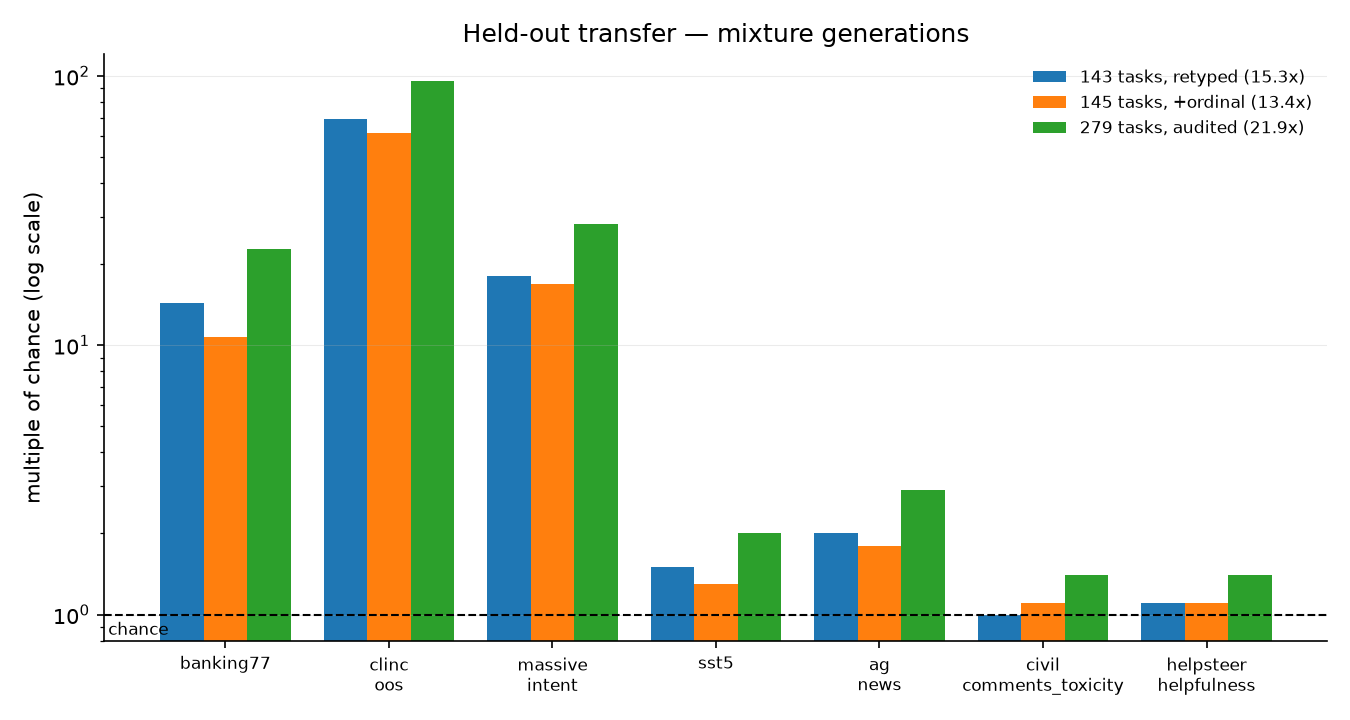
\includegraphics[width=0.95\textwidth]{figures/heldout_transfer.png}
\caption{Held-out transfer across three mixture generations, log scale,
chance marked. The middle generation is \emph{worse} than the first: that
is negative transfer from a mixture change that traded away \choice{}
tasks, retained here because a plot of only the best run would imply
progress that did not happen.}
\label{fig:transfer}
\end{figure}

\subsection{What produced the transfer}
\label{sec:res-data}

Label-space augmentation is the single largest effect we measured:

\begin{center}
\begin{tabular}{lrrr}
\toprule
held-out task & $K$ & before & after \\
\midrule
\texttt{banking77}       &  77 & 0.000 & \textbf{0.205} \\
\texttt{clinc\_oos}      & 151 & 0.000 & \textbf{0.180} \\
\texttt{massive\_intent} &  60 & 0.040 & \textbf{0.305} \\
\texttt{ag\_news}        &   4 & 0.225 & 0.655 \\
\bottomrule
\end{tabular}
\end{center}

Two exact zeroes become usable numbers. You do not need datasets with
large menus; you can synthesize them. The caveat is that the mixture also
grew from 61 to 141 tasks in the same change, so scale and shape are not
separated in this pair.

Scaling the audited mixture to 279 tasks took the mean from $17.6\times$
to $21.9\times$ and moved every task (Figure~\ref{fig:transfer}).

\subsection{Router: a fine-tuned small model against a zero-shot API}
\label{sec:res-router}

\paragraph{The comparison is asymmetric, in our favour, and we state it
before the numbers.} \openjev{} is fine-tuned on 395 labelled examples of
this task. The reference API is not: it has never seen this task's
training split, and produces its answers from the schema alone. This is
not a like-for-like contest, and a reader should discount it accordingly.
What it establishes is narrower than ``we beat Jev'': \emph{if you can
label a few hundred examples, a 1.7B open model reaches and passes a
closed API operating zero-shot on the same task.} That is a claim about
the value of labels as much as about either model.

\begin{table}[t]
\centering
\begin{tabular}{lrrrrrl}
\toprule
 & \openjev{} & reference & $b_{10}$ & $b_{01}$ & $p$ & winner \\
 & \emph{fine-tuned} & \emph{zero-shot} & & & & \\
\midrule
intent                        & \textbf{0.979} & 0.941 & 14 &  1 & 9.8e-04 & \openjev{} \\
multi-label exact set         & \textbf{0.909} & 0.822 & 57 & 18 & 7.2e-06 & \openjev{} \\
scope gate                    & \textbf{0.978} & 0.880 & 49 &  5 & 3.9e-10 & \openjev{} \\
clinical gate                 & 0.987 & 0.978 &  7 &  3 & 0.34 & level \\
abusive gate                  & 0.993 & 0.996 &  2 &  3 & 1.00 & level \\
injection gate                & 0.993 & 0.996 &  1 &  2 & 1.00 & level \\
\quad \texttt{compound\_3} tier & 0.903 & 0.645 & 11 &  3 & 0.057 & level \\
oblique clinical recall       & 0.966 & 0.793 &  5 &  0 & 0.063 & level \\
\bottomrule
\end{tabular}
\caption{Rank-16 LoRA on Qwen3-1.7B, 395 training examples, 258 seconds,
paired on the same 450 test items with exact McNemar. \openjev{} is
fine-tuned; the reference is zero-shot. Three wins, five ties, no losses.
The last two rows have $n{=}31$ and $n{=}29$, where even a large margin
struggles to reach significance: the oblique-clinical tier floors at
$p = 0.0625$ with zero losses.}
\label{tab:router}
\end{table}

\paragraph{Two rows that look like wins are not.} The
\texttt{compound\_3} tier ($0.903$ against $0.645$) and oblique clinical
recall ($0.966$ against $0.793$) are both large margins that fail the
significance test, at $p = 0.057$ and $p = 0.063$, because the tiers hold
31 and 29 items. We report them as level. They are the two tiers we most
expected to win, which is exactly why they need the test rather than the
margin.

\texttt{compound\_3} is nonetheless where the \noul{} primitive earns its
place in design terms: three simultaneous intents in one message, which a
single \choice{} softmax cannot express at all, whatever the $p$-value on
31 items says.

\paragraph{The smallest configuration is the best one.}

\begin{center}
\begin{tabular}{lrrr}
\toprule
configuration & intent & trainable & artifact \\
\midrule
encoder, all open            & 0.899 & 150M & 0.6 GB \\
decoder, head only           & 0.666 & 4.2M & 17 MB \\
decoder, all open            & 0.929 & 1{,}725M & 3.4 GB \\
\textbf{decoder, LoRA $r{=}16$} & \textbf{0.979} & \textbf{17M} & \textbf{87 MB} \\
\bottomrule
\end{tabular}
\end{center}

Adapting 17M parameters beats opening 1{,}725M, at $1/39$ the artifact.
The likely explanation is the learning rate a full fine-tune tolerates:
$10^{-5}$ over six epochs of 395 examples barely moves a 1.7B model, while
LoRA at $2\times10^{-4}$ adapts quickly without disturbing the weights it
rides on. Neither was tuned beyond one setting, so this is ``adapters are
the right default here'' rather than a tuned optimum.

\paragraph{Intermediate-task transfer.} Starting the encoder specialist
from a general checkpoint rather than raw weights, with identical data and
schedule, moves intent $0.544 \to 0.899$ and multi-label $0.453 \to 0.789$
($p = 6\mathrm{e}{-18}$). Two safety gates that never fired at all from
scratch reach $0.857$ and $0.583$ recall. This is the small-target-data
regime where STILTs predicts the largest gain.

\paragraph{But the general checkpoint was not needed here.} The $0.979$
LoRA used no mixture training at all; it started from base Qwen3-1.7B. The
general checkpoint earns its keep on schemas you have no labels for, not
on the task you actually care about.

\subsection{Latency}
\label{sec:res-latency}

\begin{center}
\begin{tabular}{lrrr}
\toprule
 & p50 & p95 & vs encoder \\
\midrule
encoder, 150M             & 37.7 ms & 50.9 ms & -- \\
decoder LoRA, unmerged    & 74.0 ms & 110.5 ms & 1.96$\times$ \\
decoder LoRA, merged      & \textbf{40.4 ms} & \textbf{55.9 ms} & \textbf{1.07$\times$} \\
\bottomrule
\end{tabular}
\end{center}

Measured back to back under identical load; read the ratios rather than
the absolute values. An unmerged adapter costs roughly $2\times$ for
nothing, since it is an extra matmul per target module at every layer.
Merged, a model eleven times larger runs 7\% slower.

\begin{figure}[t]
\centering
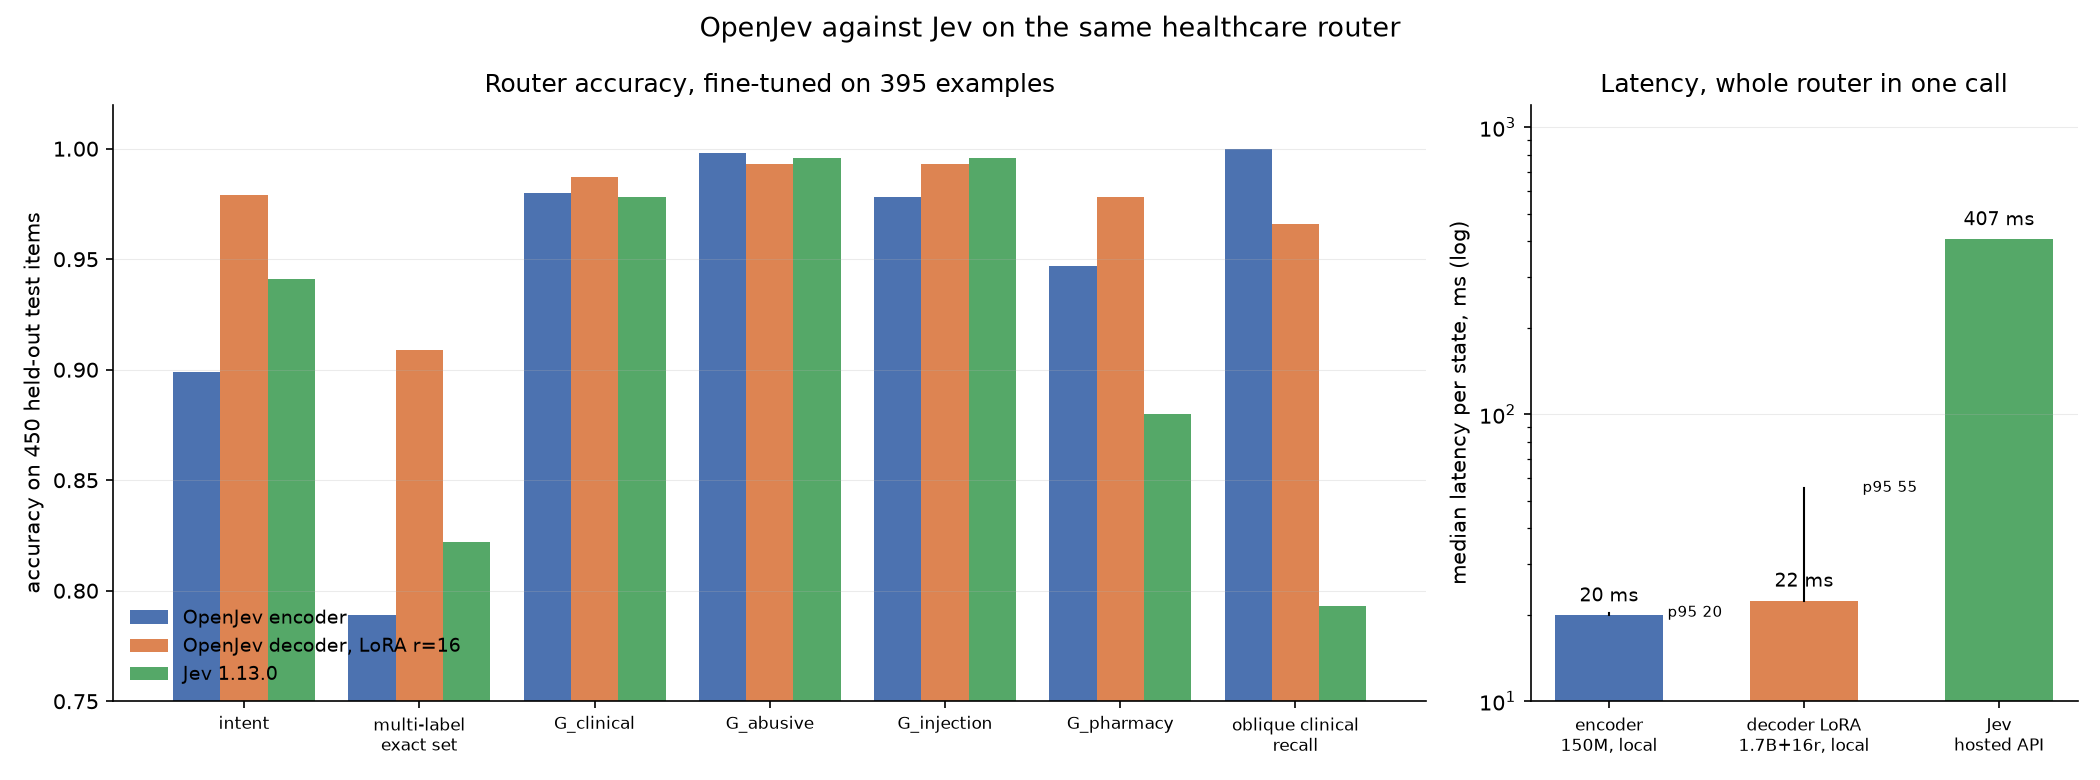
\includegraphics[width=\textwidth]{figures/comparison_router.png}
\caption{\openjev{} against the reference API on the router. Accuracy
left, latency right. The latency panel is not like-for-like: our figures
are local GPU compute and the reference is an end-to-end hosted call
including network, so it is the latency a user experiences rather than a
claim about their model's speed.}
\label{fig:comparison}
\end{figure}

\subsection{Benchmark transfer is not deployment readiness}
\label{sec:res-deployment}

The general checkpoint scores $21.9\times$ chance on the held-out suite.
Applied zero-shot to the routing task:

\begin{center}
\begin{tabular}{lrrr}
\toprule
 & zero-shot & fine-tuned & reference, zero-shot \\
\midrule
intent                & 0.601 & 0.902 & \textbf{0.941} \\
multi-label exact set & 0.427 & 0.789 & \textbf{0.822} \\
clinical gate recall  & \textbf{0.111} & 0.991 & 0.926 \\
\bottomrule
\end{tabular}
\end{center}

Intent at $0.601$ on a six-way menu is genuinely above chance, so the
transfer is real. It is also 34 points behind the reference, and the
clinical gate fires on one in nine of the cases it should catch, which is
not a gate. Clearing chance on academic benchmarks with clean label sets
is a materially weaker claim than working on a deployment task you have no
labels for, and the two come apart sharply here. Safety gates in
particular appear to require task supervision.
